\section{System Description}
\subsection{Go-Kart Frame}
The Go-Kart itself consists of a pre assembled steel frame with wheels, steering column, break pedal and seat all pre attached to the frame.

from \todo{company name / model nr of gokart?}

The Go-Kart fits one regular adult in the seat.

Behind the seat a plate is attached to fit all power electronics and drive systems produced in this project.

The Go-Kart has a pre installed break pedal attached to a disc break by a mechanical system of springs. \todo{expand and take a picture of this}.

The wheels are \todo{inches? rubber? needed?}


\begin{figure}[!h]
	\centering
	\missingfigure{pic of kart}
	%\includegraphics[width=.85\linewidth]{graphics/wiringdiagram}
	\caption{Picture of the go kart frame}
	\label{fig:Kart_picture1}
\end{figure}


\subsection{Battery Supply}
The batteries provided for this project are called: "SB12V20P-FC Super B
Lightweight Lithium Ion starter battery". \todo{cite datasheet}
Four of these batteries will be combined in a single supply package yielding a combined nominal voltage of 52.8V and a discharge current of 560A. The discharge current can go up to as much as 1200A for a single second of pulse.
The batteries are relatively  small at $\approx 238x120x82mm$ and $3.2kg$ of weight each.
This battery pack will be providing all he required power for the Go-kart, including the motor and all control and drive circuits.




\subsection{PMAC Motor}

\subsection{Torque Pedal}
The torque pedal or "speeder" is provided as well. It consists of a levered variable resistor with the equivalent diagram seen on figure \ref{fig:Torque_pedal_diagram}.

The torque pedal will be used to control the speed by increasing or lowering the resistance, resulting in a change of voltage on the return wires. Measuring the pedal, it is found to have a variable resistance of 0k to 7.5k. It is also found to be inaccurate while holding a position, meaning some kind of filter will be necessary.

\begin{figure}[!h]
	\begin{subfigure}[t]{.35\linewidth}
			\centering
			\includegraphics[width=\textwidth]{graphics/torque_pedal_diagram}
			\caption{Diagram of the torque pedal}
			\label{fig:Torque_pedal_diagram}
	\end{subfigure}
	\hspace{2cm}
	\begin{subfigure}[t]{.35\linewidth}
		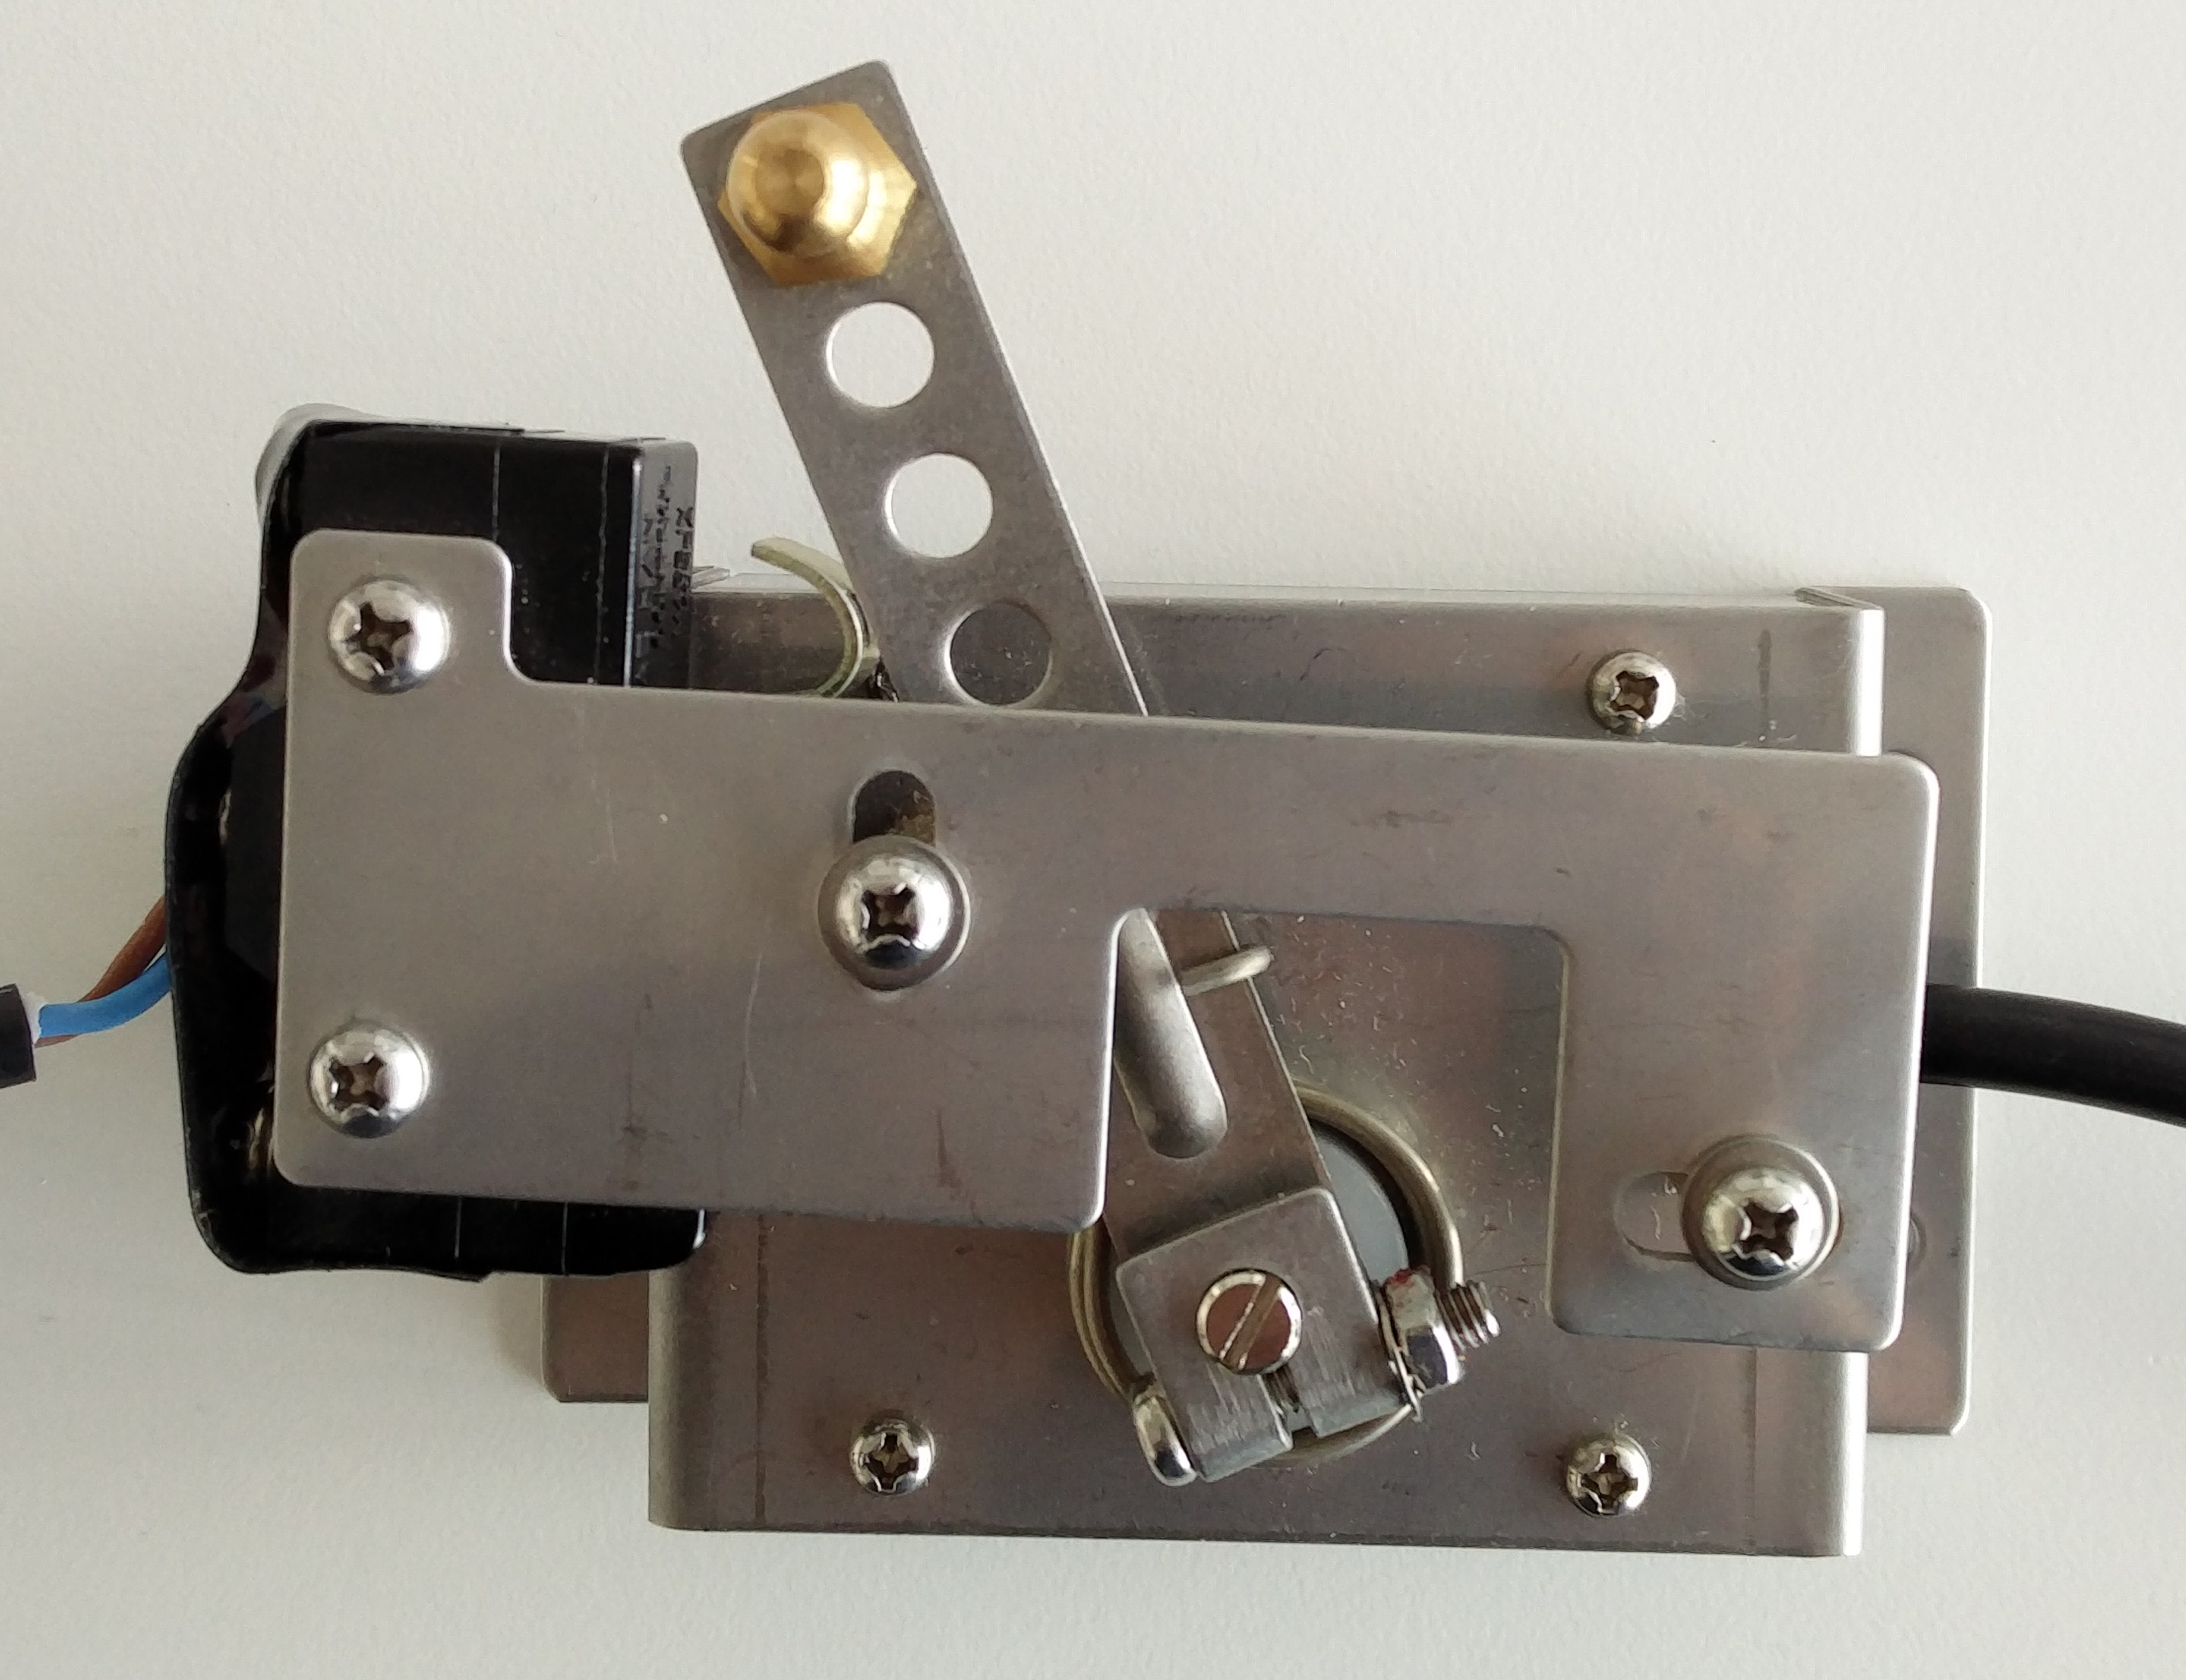
\includegraphics[width=\textwidth]{graphics/torque_pedal_picture}
		\caption{Picture of the actual torque pedal}
		\label{fig:Torque_pedal_picture}
	\end{subfigure}
	\caption{Diagram and picture of the torque pedal}
	\label{fig:Torque_pedal_diagram}
\end{figure}
\todo{align pictures, maybe cut out the background of the pedal}


\subsection{Switches and Wireing}
The wiring of the Go-Kart frame is not pre Assembled with it, but has been provided by supervisors of the project, as this is standardized across multiple projects.

A diagram of the wiring can be seen below.

\todo{create wiring diagram of the Go-Kart}



\clearpage